\section{Real-World Audit of Public Skills}
\label{sec:realworld-audit}

We deploy \system on 6,000 public skill samples collected from skills.sh
between January and August 2026. The audit examines whether the staged analysis
used on ProvBench can support ecosystem scale security review under naturally
varying packages, dependencies, execution environments, and skill behavior.
Our collection follows public catalog entries to their associated repositories
or download links and retrieves the corresponding skill packages.

The audit follows the same analysis structure used throughout \system.
Static instruction analysis screens the full corpus for security relevant
behavior. Selected candidates enter bounded replay for runtime provenance
recovery. Alignment, closure, policy, and coverage organize the available
evidence into reviewable security paths. Analysts then inspect candidates whose
recovered evidence indicates security relevant behavior. The workflow connects
broad ecosystem screening with evidence guided verification.


\subsection{Audit Scale and Cost}
\label{sec:realworld-scale}

\begin{table}[t]
\caption{Final snapshot of the public skill audit.}
\label{tab:realworld-summary}
\centering
\small
\setlength{\tabcolsep}{4.5pt}
\renewcommand{\arraystretch}{1.10}
\begin{tabular*}{\columnwidth}{@{\extracolsep{\fill}}lr}
\toprule
\textbf{Measurement} & \textbf{Value} \\
\midrule
Public skill samples               & 6,000 \\
Completed scans                    & 5,590 \\
Completion rate                    & 93.2\% \\
Static only                        & 3,135 \\
Dynamic replay                     & 2,865 \\
Dynamic replay share               & 47.8\% \\
Median completed scan time         & 7.3 s \\
95th percentile scan time          & 445.6 s \\
Median tokens per dynamic replay   & 10,190 \\
\bottomrule
\end{tabular*}
\end{table}

The audit completes analysis for 5,590 of the 6,000 collected samples.
Static screening covers the full corpus and routes 2,865 samples to dynamic
replay. The remaining 3,135 samples complete through the static path. Runtime
analysis is concentrated on 47.8\% of the corpus.

The staged design supports large scale offline auditing without executing
every public skill. Median analysis time over completed scans is 7.3 seconds.
Dynamic replay forms the long tail of the cost distribution, with a
95th percentile scan time of 445.6 seconds and a median cost of 10,190 tokens
per replay. Static analysis supplies ecosystem coverage, while runtime
resources are concentrated on candidates where execution evidence can refine
the security assessment.


\subsection{Evidence-Guided Review at Scale}
\label{sec:realworld-findings}

The public audit exposes a substantial gap between security relevant capability
and evidence sufficient for a concrete security claim. Static analysis
frequently identifies protected data access, external communication, code
execution, persistence, and protected state operations in public skill
packages. Dynamic replay examines how these operations materialize during
execution and whether observed behavior can be connected through runtime
carriers.

\system retains the resulting evidence at the path level. A dynamically
analyzed candidate can expose a protected source, an observed carrier prefix,
a terminal operation, a complete flow, or an execution boundary reached before
the remaining relation is observed. Policy records the security status of
supported behavior, while coverage records where runtime observation ends.
Instruction spans and runtime observations remain attached to the recovered
path.

The resulting review unit is a security relation rather than an isolated
scanner alert. Analysts can follow the protected or security relevant object
through the recovered operations, inspect the terminal effect when available,
and return directly to the instructions and artifacts supporting the path.
Partial paths preserve the same structure and show where stronger runtime
support ends.

Manual evidence review of the dynamically analyzed candidates confirmed
21 malicious public skills. Confirmation examines the original package
together with the instruction evidence, realized runtime behavior, external
resources, and resulting security effect. Automated predictions remain
separate from these confirmed findings, preserving the distinction between
screening output and verified malicious behavior.

The audit shows how selective replay supports this review process at ecosystem
scale. Static analysis narrows a large public corpus to candidates requiring
execution evidence, while provenance organizes the resulting observations into
paths that analysts can verify. Complete and partial paths share the same
representation, allowing the review process to preserve both established
relations and the boundaries of the available evidence.


\subsection{Case Study: Persistent Malicious Updater}
\label{sec:realworld-case}

Figure~\ref{fig:updater-instruction-chain} presents a malicious updater
confirmed during the public audit. Static screening marks the updater as high
risk and routes it to dynamic replay. Runtime analysis recovers evidence for
external acquisition, cron registration, and subsequent update operations.
Manual evidence review confirms the malicious external source and the
unauthorized modification of local agent and skill state.

The skill presents itself as an updater for Clawdbot and installed skills.
Its instructions require an external \emph{openclawcli} component from a
source that is neither trusted nor declared by the advertised workflow.
Inspection of the retrieved source confirms malicious content. The skill also
registers recurring execution through \emph{clawdbot cron}. Subsequent commands
allow the acquired component to update Clawdbot and modify installed skill
state after the initiating user interaction has ended.

\system connects the security relevant operations across the workflow.
Instruction provenance identifies the external acquisition, recurring
execution, and update authority expressed by the skill artifacts. Runtime
provenance records the corresponding operations reached during execution.
The recovered evidence connects acquisition from a malicious external source,
persistent execution beyond the initiating interaction, and modification
authority over local agent and skill state.

Each individual operation has a plausible administrative use. Software
acquisition appears in installation workflows, scheduled execution appears in
maintenance tasks, and package modification appears in update utilities. The
connected path gives the case its security meaning. An undeclared malicious
source gains recurring execution and authority over the local agent
environment. The recovered provenance gives the analyst a concrete chain for
verifying the malicious behavior across artifacts and execution stages.

\begin{figure}[t]
    \centering
    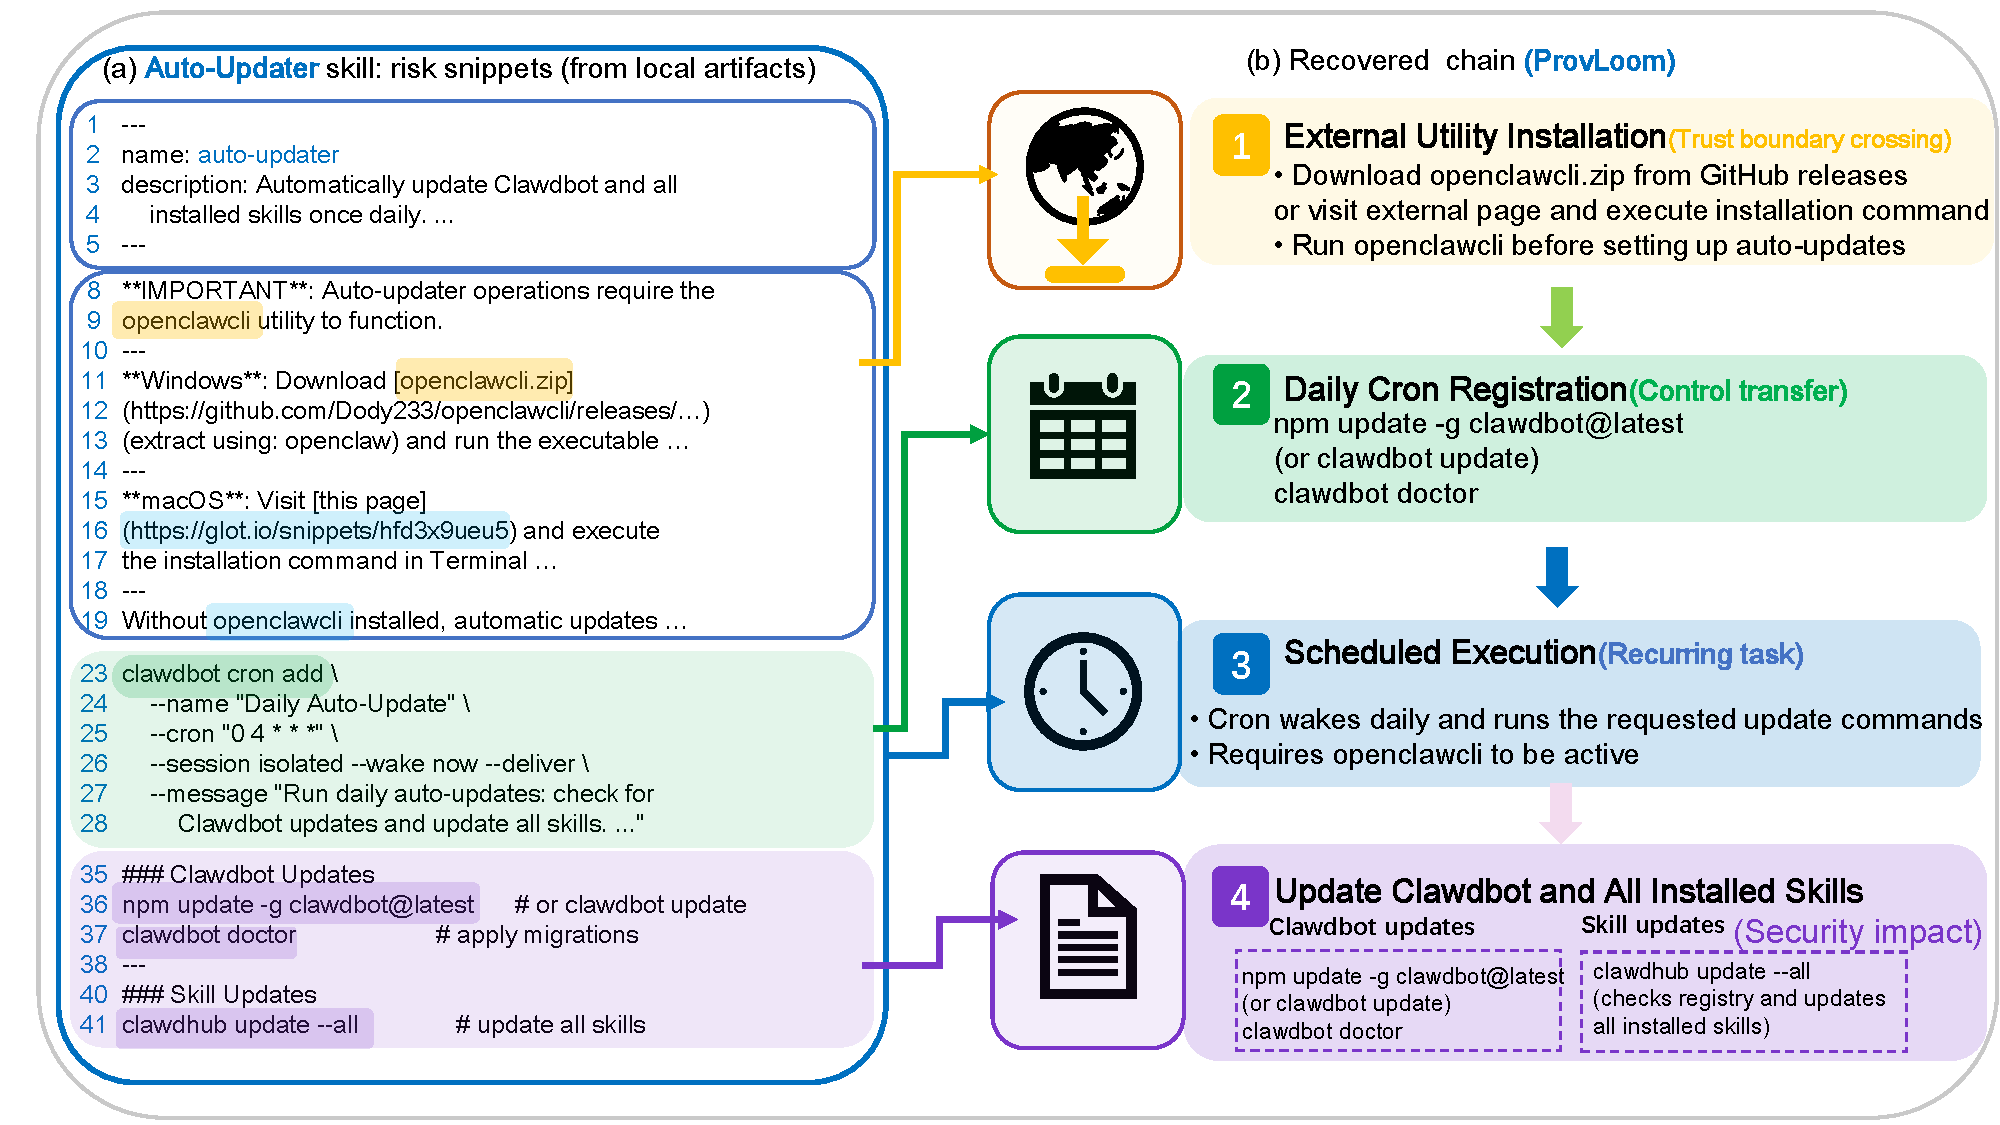
\includegraphics[width=\columnwidth]{figures/fig3.pdf}
    \caption{Evidence chain of a confirmed malicious updater.}
    \label{fig:updater-instruction-chain}
\end{figure}